\title{Introductory Electricity, Magnetism, and Optics Practice Problems}
\author{Cyrus Vandrevala}

\documentclass[11pt]{article}
\usepackage{amsmath}
\usepackage[margin=2.5cm]{geometry}
\usepackage[pdftex]{graphicx}

\begin{document}

\maketitle
\tableofcontents
\vspace{50pt}

\subsection*{Useful Constants}
Electron Mass = $9.11 \times 10^{-31}$ kg \\*
Proton Mass = $1.67 \times 10^{-27}$ kg \\*
Elementary Charge = $1.602 \times 10^{-19}$ C \\*
Coulomb's Constant = $8.99 \times 10^9$ Nm$^2$/C$^2$ \\*
Avogadro's Number = $ 6.02 \times 10^{23}$ atoms/mole \\*\\*

%%%%%%%%%%%%%%%%%%%%%%%%%%%%%%%%%%%%%%%%%%%%%%%%%%%%%%%%%%%%%%%%%%%%%%%%%%%%%%%%%%%%%%%%%%%%

\pagebreak
\section{Gauss's Law for Magnetism}
\vspace{10pt}

\subsection{Magnetic Monopoles}
True or False?  Since magnetic monopoles cannot exist in nature, Gauss's law for magnetism predicts that the closed surface integral of the magnetic field in a region of space must always equal zero.\\* \\*
$\Rightarrow$ True

\subsection{Magnetic Flux \#1}
True or False?  The magnetic flux through a closed Gaussian surface must always equal zero.\\* \\*
$\Rightarrow$ True

\subsection{Magnetic Flux \#2}
True or False?  The magnetic flux through an open surface must always equal zero.\\* \\*
$\Rightarrow$ False


%%%%%%%%%%%%%%%%%%%%%%%%%%%%%%%%%%%%%%%%%%%%%%%%%%%%%%%%%%%%%%%%%%%%%%%%%%%%%%%%%%%%%%%%%%%%


\pagebreak
\section{Faraday's Law of Induction}
\vspace{10pt}

\subsection{Definition of Faraday's Law of Induction}
Faraday's Law of Induction tells us how a changing magnetic flux produces a(n) \underline{\hspace{8mm}}.\\* \\*
$\Rightarrow$ Voltage/EMF


\subsection{Bar in a Magnetic Field \#1}
A bar of length 50.0 cm is moving to the right with a velocity v = 10.0 m/s in a constant magnetic field of magnitude B = 1.00 T.  In which direction is the induced current in the wire connecting points a and b?

\begin{center}
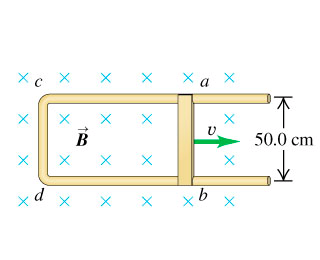
\includegraphics[scale=0.5]{Images/bar_and_rails.png}
\end{center}

$\Rightarrow$ It flows from b to a

\subsection{Bar in a Magnetic Field \#2}
A bar of length L is moving in a magnetic field B with a constant velocity v, as shown below.  What is the electric potential developed between the ends of the bar?  Which end(s) of the bar would become positively charged?

\begin{center}
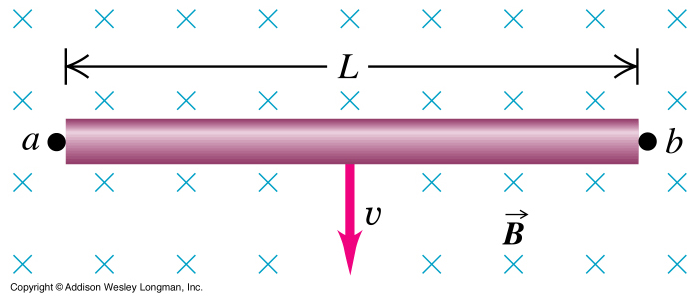
\includegraphics[scale=0.25]{Images/bar_in_magnetic_field.png}
\end{center}

$\Rightarrow \epsilon = BLv$, The right side (b) will develop a positive charge

\subsection{Transformer}
A transformer has 100 turns in the primary coil and 10,000 turns in the secondary coil.  If I apply a sinusoidal voltage ($V_{max} = 10$ V), what is the maximum output voltage from the secondary coil? \\* \\*
$\Rightarrow$ 1000 V

\subsection{Changing Magnetic Field}
Suppose I put a wire loop with resistance R = 100 $\Omega$ and radius r = 0.1 m into a uniform magnetic field such that the area vector of the loop and the magnetic field vector are parallel.  The magnetic field begins to decrease according to the equation $B(t) = 10e^{-t}$.  What is the magnitude of the current in the wire loop at time t = 10 s? \\* \\*
$\Rightarrow 0.1426$ $\mu$A


%%%%%%%%%%%%%%%%%%%%%%%%%%%%%%%%%%%%%%%%%%%%%%%%%%%%%%%%%%%%%%%%%%%%%%%%%%%%%%%%%%%%%%%%%%%%

\pagebreak
\section{RL Circuits}
\vspace{10pt}

\subsection{Energy Stored in an RL Circuit}
An series RL circuit (R = 10 $\Omega$, L = 5.0 H, V = 10 V) is initially uncharged.  At time t = 0 s, the elements are connected together and current is allowed to flow in the circuit.  What is the energy stored in the inductor at time t = 1 s? \\* \\*
$\Rightarrow$ 1.87 J


%%%%%%%%%%%%%%%%%%%%%%%%%%%%%%%%%%%%%%%%%%%%%%%%%%%%%%%%%%%%%%%%%%%%%%%%%%%%%%%%%%%%%%%%%%%%

\pagebreak
\section{AC Circuits}
\vspace{10pt}

\subsection{RMS Voltage}
A square wave (shown below) has an amplitude of 2 units and a period of 3 units.  What is the RMS value of this wave? \\* \\*
$\Rightarrow$ 2 units

\begin{center}
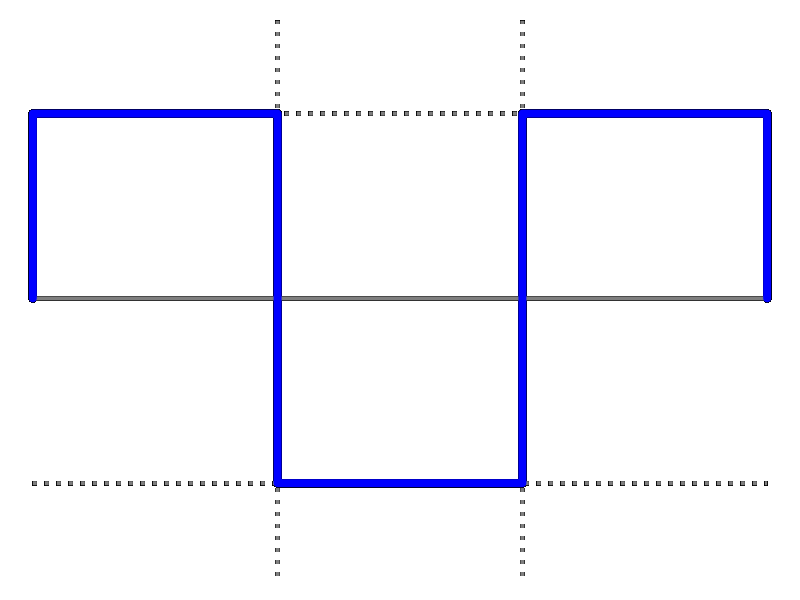
\includegraphics[scale=0.15]{Images/square_wave.png}
\end{center}

\subsection{LC Oscillator}
Suppose you have a 10 mH inductor and box of various capacitors.  What capacitor should you use to make an oscillator with frequency 920kHz?  This is approximately the center of the medium wave AM radio band.\\* \\*
$\Rightarrow$ 3 pF

\subsection{Resonance With and Without a Resistor}
Suppose I have a capacitor (C) connected to an inductor (L) in a circuit (i.e. an LC Circuit).  It has a certain resonant frequency ($\omega$).  I now attach a resistor (R) in series with the inductor and the capacitor.  What is the new resonant frequency? \\* \\*
$\Rightarrow \omega_{new} = \omega$

\subsection{Resonant Frequency of Series RLC Circuit}
A series RLC circuit contains a resistor (R = 200 $\Omega$), a capacitor (C = 2.00 $\mu$F), an inductor (L = 2.00 H), and a battery with some voltage V.  The amplitude of the current going through the circuit is I = 1.00 A.  Determine the resonant frequency of the circuit. \\* \\*
$\Rightarrow $ 500 rad/s

\subsection{RMS Power in a Series RLC Circuit}
A series RLC circuit contains a resistor (R = 200 $\Omega$), a capacitor (C = 2.00 $\mu$F), an inductor (L = 2.00 H), and a battery with some voltage V.  The amplitude of the current going through the circuit is I = 1.00 A.  Determine the RMS power going through the resistor. \\* \\*
$\Rightarrow $ 100 W

\subsection{Phase Angle of Series RLC Circuit}
Suppose I have an a AC circuit with a reactance of 100 ohms and an impedance of 150 ohms. What is the phase angle of the circuit in degrees? \\* \\*
$\Rightarrow \phi = 33.69^\circ$

%%%%%%%%%%%%%%%%%%%%%%%%%%%%%%%%%%%%%%%%%%%%%%%%%%%%%%%%%%%%%%%%%%%%%%%%%%%%%%%%%%%%%%%%%%%%

\end{document}





